% --- FIGURE 4: TASK SUCCESS COMPARISON (BAR CHART) ---
% Saved in assets/fig_success_bar.tex

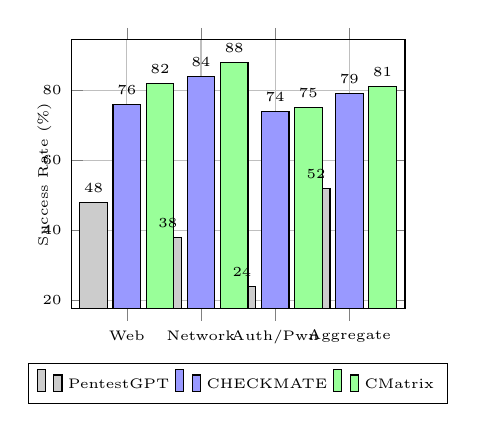
\begin{tikzpicture}
\begin{axis}[
    ybar,
    enlarge x limits=0.25,
    legend style={at={(0.5,-0.2)}, anchor=north, legend columns=-1, font=\tiny},
    ylabel={Success Rate (\%)},
    symbolic x coords={Web, Network, Auth/Pwn, Aggregate},
    xtick=data,
    nodes near coords,
    nodes near coords align={vertical},
    bar width=10pt,
    width=0.48\textwidth,
    height=5cm,
    font=\tiny,
    ylabel style={yshift=-10pt},
    grid=major,
    ymajorgrids=true,
]

% PentestGPT (USENIX '24)
\addplot[fill=gray!40] coordinates {(Web,48) (Network,38) (Auth/Pwn,24) (Aggregate,52)};

% CHECKMATE (USENIX '25 SOTA)
\addplot[fill=blue!40] coordinates {(Web,76) (Network,84) (Auth/Pwn,74) (Aggregate,79)};

% CMatrix (Ours)
\addplot[fill=green!40] coordinates {(Web,82) (Network,88) (Auth/Pwn,75) (Aggregate,81)};

\legend{PentestGPT, CHECKMATE, CMatrix}
\end{axis}
\end{tikzpicture}

% --- FIGURE 5: LONGITUDINAL MEMORY GAIN (LINE GRAPH) ---
% Saved in assets/fig_memory_gain.tex

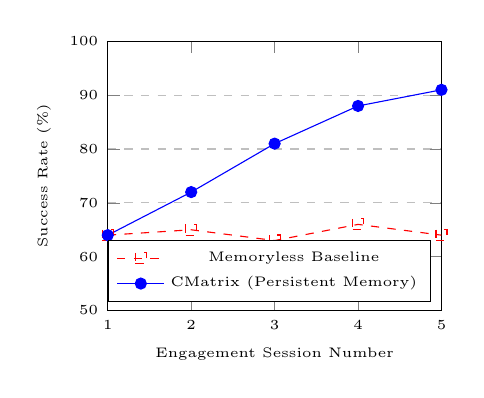
\begin{tikzpicture}
\begin{axis}[
    xlabel={Engagement Session Number},
    ylabel={Success Rate (\%)},
    xmin=1, xmax=5,
    ymin=50, ymax=100,
    xtick={1,2,3,4,5},
    ytick={50,60,70,80,90,100},
    legend pos=south east,
    legend style={font=\tiny},
    ymajorgrids=true,
    grid style=dashed,
    width=0.48\textwidth,
    height=5cm,
    font=\tiny
]

% Baseline (No Memory)
\addplot[
    color=red,
    mark=square,
    dashed
    ]
    coordinates {
    (1,64)(2,65)(3,63)(4,66)(5,64)
    };
    \addlegendentry{Memoryless Baseline}

% CMatrix (Agentic RAG + Reranking)
\addplot[
    color=blue,
    mark=*,
    ]
    coordinates {
    (1,64)(2,72)(3,81)(4,88)(5,91)
    };
    \addlegendentry{CMatrix (Persistent Memory)}

\end{axis}
\end{tikzpicture}
